
\section{Results}
\label{sec:results}
This section presents the results of our empirical evaluation and answers, one by one, our research questions.

\subsection{Best MOEA for \moho (RQ1)} 
\label{sec:results:rq1}

\begin{table} [t]
    \centering
    \caption{MOEAs ranking (in \moho) in  terms of crash reproduction ratio (Friedman's test) and results of the pairwise comparison ($p$-value $\leq$ 0.05)}
    \label{tab:internal-assessment}
    % \begin{smaller}
    \begin{tabular}{ r l c l}
\hline
    \textbf{Rank} & \textbf{MOEA} & \textbf{Rank value} & \textbf{Significantly better than} \\
    \hline
    1    & SPEA2    & 2.63    & (2), (3), (4), (5) \\
    2    & PESA-II  & 2.86    & (4), (5) \\
    3    & NSGA-II  & 2.90    & (4), (5) \\
    4    & MOEAD    & 4.97    & (5) \\
    5    & FEMO     & 5.05    &  \\
    \hline
    \end{tabular}
    % \end{smaller} 
\end{table}

\begin{figure}[t]
    \centering
    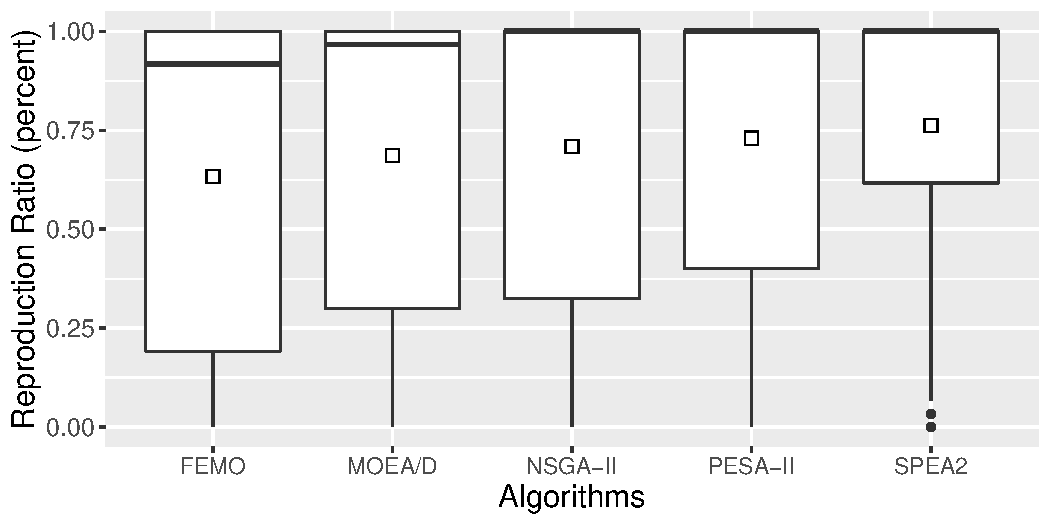
\includegraphics[width=\linewidth]{papers/moho/figures/reproduction-overall.pdf}
    % \Description{A boxplot presenting the crash reproduction ratio of the different algorithms when using MO-HO.}
    \caption{Crash reproduction ratio (out of 30 executions) of \moho algorithms.  The upper and lower edge of each box present the upper and lower quartile, respectively. ($\square$) denotes the arithmetic mean and (---) is the median.}
    \label{fig:eval:results-rq1-overall}
\end{figure}

Figure \ref{fig:eval:results-rq1-overall} presents the crash reproduction ratio of the MOEAs applied to our \moho framework. For this analysis, we consider the number of times (in percentage) each MOEAs could reproduce a given crash across 30 runs and using a search budget of five minutes. On average (the squares in Figure \ref{fig:eval:results-rq1-overall}), the best algorithm for \moho is  \textit{SPEA2}, with an average and median of $76\%$ and $100\%$ of successful reproductions, respectively. \textit{SPEA2} is Followed by \textit{PESA-II}, \textit{NSGA-II}, and \textit{MOEAD}. Also, this figure shows that the first quartile of the crash reproduction ratio of \textit{SPEA2} is, at least, about 25\% higher than other MOEAs.

According to Friedman's test, the differences in reproduction ratios are statistically significant ($p$-value $\leq$ $0.05$).
This means that some MOEAs are significantly better than others within our \moho framework.  For completeness, Table~\ref{tab:internal-assessment} reports the
ranking produced by the Friedman test. To better understand for which
pairs of MOEAS the statistical significance holds, we applied the post-hoc Conover's procedure for the pairwise comparison. The results of the comparison are also reported in Table~\ref{tab:internal-assessment}.
According to this table, the best-performing algorithm is \moho + \textit{SPEA2}, which has a significantly higher crash reproduction ratio compared to other \moho algorithms. The next algorithms are \moho + \textit{PESA-II} and \moho + \textit{NSGA-II}. These two algorithms are significantly better than \moho + \textit{MOEAD} and \moho + \textit{FEMO}. Finally, the worst algorithm in terms of crash reproduction is \textit{FEMO}, which is significantly worse than other MOEAs.


\textbf{Summary (RQ$_1$). } \textit{\moho + \textit{SPEA2} achieved the highest performance in terms of crash reproduction ratio compared to \moho + other MOEAs. 
The next best-performing MOEAs, in terms of crash reproduction, are \textit{PESA-II} and \textit{NSGA-II}.
}

\subsection{Crash Reproduction (RQ2)} 
\label{sec:results:rq2}

\begin{figure*}[t]
    \centering
    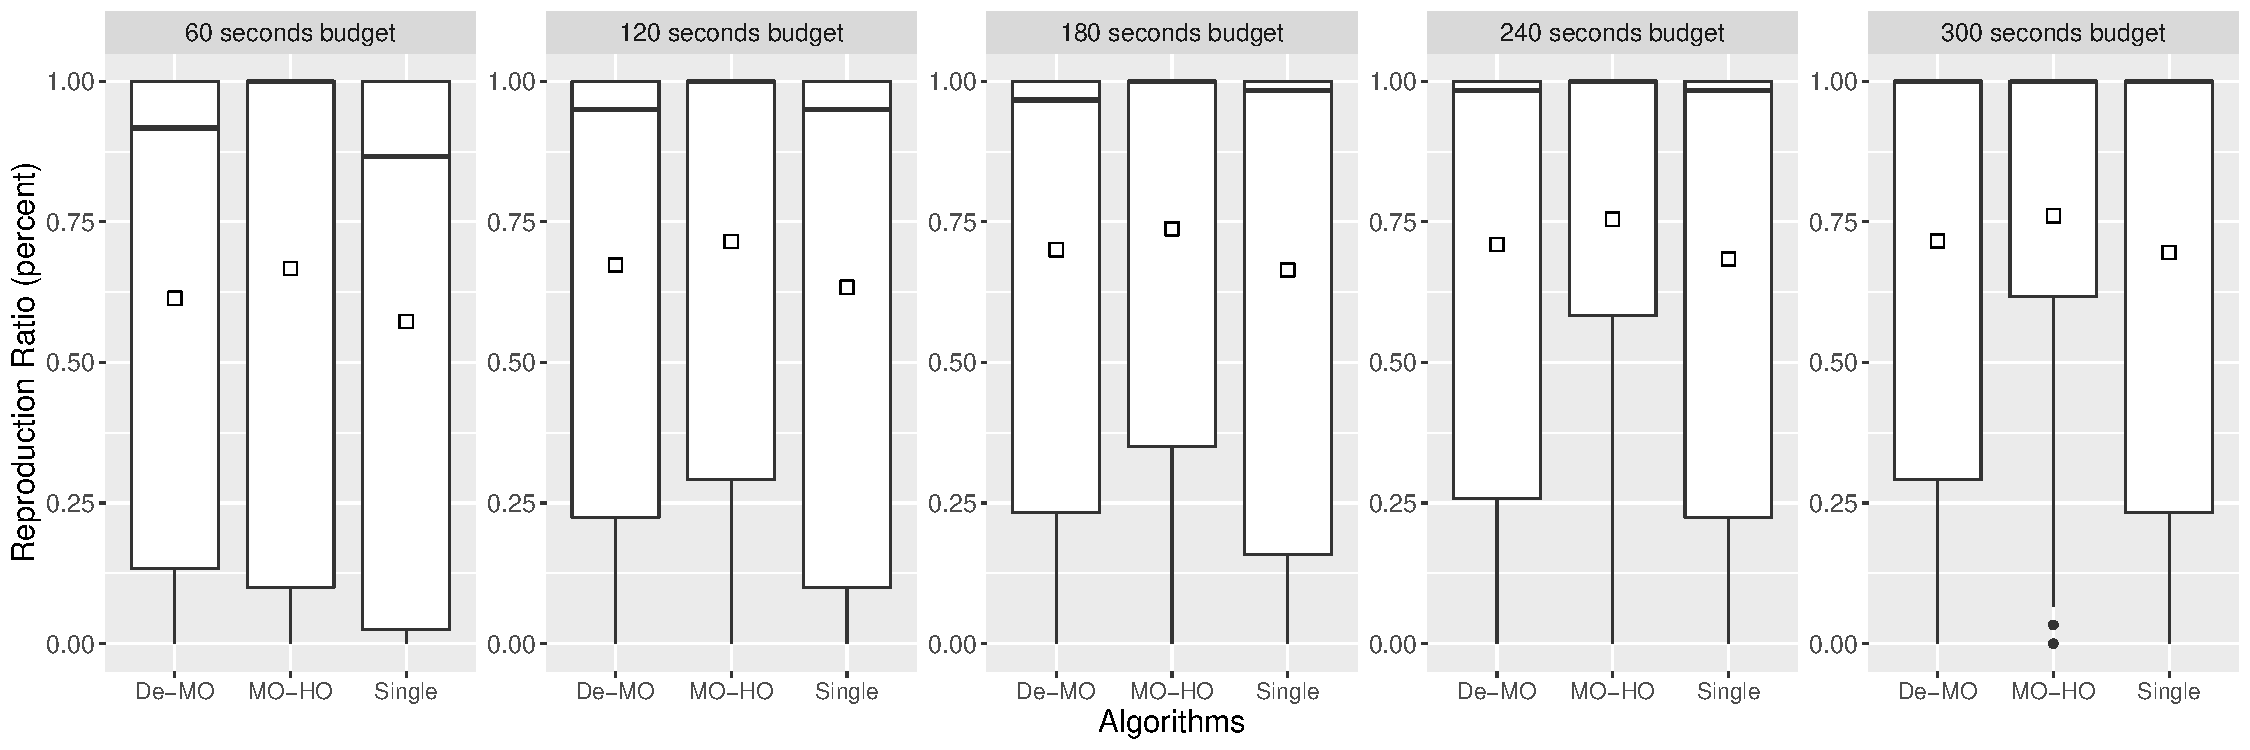
\includegraphics[width=\linewidth]{papers/moho/figures/rq2-reproduction-overall.pdf}
    % \Description{A boxplot presenting the crash reproduction ratio of MO-HO, Single and De-MO for five different time budgets.}
    \caption{Crash reproduction ratio (out of 30 executions) of \moho against state-of-the-art in five different time intervals.  ($\square$) denotes the arithmetic mean and (---) is the median.}
    \label{fig:eval:reproduction-rq2}
\end{figure*}

\begin{figure}[t]
    \centering
    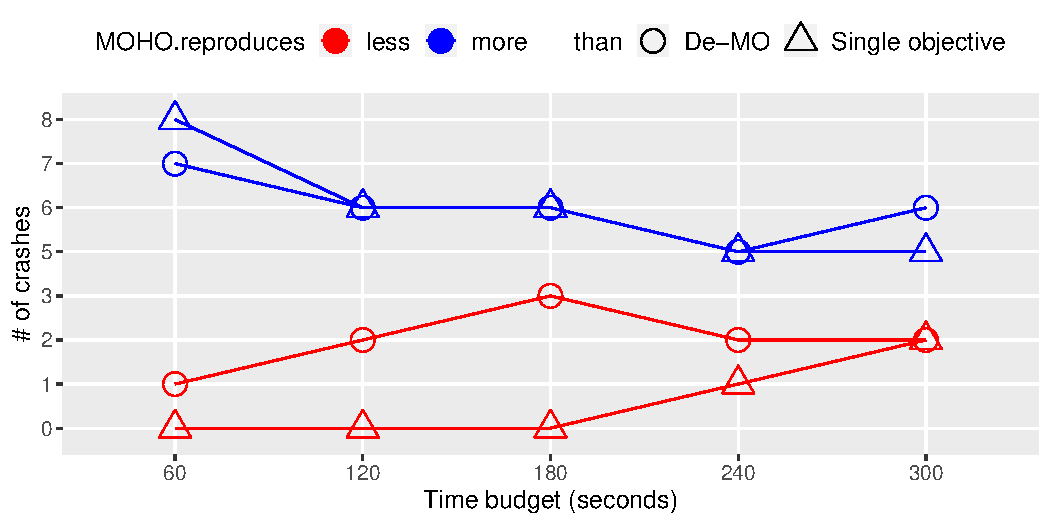
\includegraphics[width=\linewidth]{papers/moho/figures/rq2-reproduced-crashes.pdf}
    % \Description{A graph presenting the number of crashes reproduced only by MO-HO, Single, or De-MO for five different time budgets.}
    \caption{Number of crashes reproduced only by \moho or only by one of the state-of-the-art algorithms.}
    \label{fig:eval:results-rq2}
\end{figure}

Figure \ref{fig:eval:reproduction-rq2} depicts the crash reproduction ratio of the best-performing \moho configuration (i.e., with \textit{SPEA2}), \SGGA, and \decomposition at five time intervals (search budgets). As indicated in this figure, the average crash reproduction ratio of \moho is higher than other algorithms at all of the time intervals. Also, the median crash reproduction ratio for this algorithm is always 100\%. Furthermore, the maximum improvement achieved by \moho with the five-minutes search budget is in \textit{XWIKI-14599} (with 100\% improvement) and \textit{MATH-3b} (with 93.3\% improvement) compared to \SGGA and \decomposition, respectively. In contrast, the largest reduction in reproduction ratio by \moho (with the five-minutes budget) is in \textit{XCOMMONS-1057} (with 30\% drop) and \textit{XWIKI-13616} (with 40\% reduction) compared to \SGGA and \decomposition, respectively. We will explain the negative factors in \moho, which lead to negative results for this algorithm in some corner cases, in Section \ref{sec:results:corner}.
 
Moreover, we can see that \decomposition is the second-best algorithm in all of the time intervals. In the first 60 seconds of the crash reproduction process, on average, its crash reproduction ratio is 4\% better than \SGGA. However, in contrast to the other two algorithms, the crash reproduction ratio of this algorithm changes only slightly after the first 120 seconds. Hence, at the end of the search process, the average crash reproduction ratio of \decomposition is only 2\% better than \SGGA. In contrast, since the crash reproduction ratio of \moho keeps growing, on average, it remains more effective than \SGGA (about 10\%) even after 300 seconds. The other interesting point in Figure \ref{fig:eval:reproduction-rq2} is the first quantile of \moho. In the first 60 seconds, this value is lower than 12\%, but it grows up to 62\% after 300 seconds. This improvement is not observable in state-of-the-art algorithms.

Furthermore, \moho is more stable in crash reproduction after 300 seconds budget compared to the other algorithms. Figure 3 demonstrates that the interquartile range (i.e., the difference between first and third quartile) of crash reproduction ratio in \moho with the 300 seconds budget is 46\% smaller than the interquartile range of other algorithms (being 38.3\% for \moho, 76.6\%. for \SGGA, and  70.8\% for \decomposition).

Also, Figure \ref{fig:eval:results-rq2} shows the number of crashes, which are reproduced by \moho, but not by the state-of-the-art algorithms and vice versa in different time intervals.
As indicated in this figure, in all of the time intervals, the number of crashes that are reproduced by \moho is higher than the crashes that it cannot reproduce. In the best case (after 1 minute of search), \moho reproduces eight and seven new crashes that cannot be reproduced by \SGGA and \decomposition, respectively. In contrast, there is only one crash that can be reproduced by \decomposition and not by \moho. Also, after five minutes, \moho still reproduces more crashes than the baselines: it reproduces five and six new crashes that cannot be reproduced by \SGGA and \decomposition, respectively.

The crashes that are reproduced by \moho after five minutes but not by \SGGA are: \texttt{TIME-10b} frame 5, \texttt{XCOMMONS-\\928} frame 2, \texttt{XWIKI-14227} frame 2, \texttt{XWIKI-14475} frame 1, and \texttt{XWIKI-14599} frame 1. And the crashes that are reproduced by \moho after five minutes but not by \decomposition are: \texttt{MOCKITO-16b} frame 4, \texttt{TIME-5b} frame 3, \texttt{XWIKI-13377} frame 3, \texttt{XWIKI-14227} frame 2, \texttt{MATH-3b} frame 1, and \texttt{MOCKITO-10b} frame 1.

Figure \ref{lst:moho:stacktracexwiki} shows the crash's stack trace reported in the issue \texttt{X\-WI\-KI-14227}. \moho is the only approach that can reproduce the first two frames of this stack trace. Here, the target method is \texttt{useMainStore} (Figure \ref{lst:xwikiframe2}), which does not have any input argument. Hence, to reproduce this crash, the crash reproducing test generated by \moho (depicted in Figure \ref{lst:generatedtest}) should invoke specific methods (\eg \texttt{setWiki}, \texttt{setWikiId}) to set different local variables in the \texttt{xwikiContext0} object, and then, pass this object to the class under test (here, \texttt{Acti\-vi\-ty\-Stream\-Con\-fi\-gu\-ra\-tion}). Since the crash reproducing  test case generated by \moho does not add any plugin to the \texttt{xWiki0} object, the execution of this test indeed leads to a \texttt{NullPointerException} thrown at line 5619 of the \texttt{getPlugin} method in Figure \ref{lst:xwikiframe1}.
Generating such a specific test case requires a search process with high exploration ability, which can generate diverse test cases.

We do note that \SGGA cannot even generate a test case covering the target line (line 85 of the \texttt{useMainStore} method). However, \decomposition can cover the target line thanks to more test generation diversity delivered by the application of multi-objectivization.

\begin{figure}[t]
    \begin{lstlisting}[numbers=left,
        firstnumber=0]
java.lang.NullPointerException: null
	at [...].XWiki.getPlugin(XWiki.java:5619)
	at [...].ActivityStreamConfiguration.useMainStore([...]:85)
    [...]
    \end{lstlisting}
    % \Description{The stack trace from the XWIKI-14227 crash, composed of a thrown NullPointerException and the list of frames describing the active stack of method calls through which the exception propagated.}
    \caption{XWIKI-14227 crash's stack trace.}
    \label{lst:moho:stacktracexwiki}
\end{figure}

\begin{figure}[t]
    \begin{lstlisting}[numbers=left,
        firstnumber=82,
        language=Java,
        basicstyle=\footnotesize]
public boolean useMainStore(){
    XWikiContext context = contextProvider.get();
    if (context.isMainWiki()) {return false;}
    ActivityStreamPlugin plugin = (ActivityStreamPlugin) context.getWiki().getPlugin[...] context); // <-- target line 
}
    \end{lstlisting}
    % \Description{A code excerpt of the useMainStore method mentioned in the XWIKI-14227 crash.}
    \caption{Method \texttt{useMainStore} appears in the second frame of the \texttt{XWIKI-14227} crash's stack trace.}
\label{lst:xwikiframe2}
\end{figure}
    
\begin{figure}[t]
    \begin{lstlisting}[numbers=left,
            firstnumber=5617,
            language=Java,
            basicstyle=\footnotesize]
public XWikiPluginInterface getPlugin([...]){
    XWikiPluginManager plugins = getPluginManager();
    Vector<String> pluginlist = plugins.getPlugins();
    [...]
}
    \end{lstlisting}
    % \Description{A code excerpt of the getPlugin method mentioned in the XWIKI-14227 crash.}
    \caption{Method \texttt{getPlugin} appears in the first frame of the \texttt{XWIKI-14227} crash's stack trace.}
    \label{lst:xwikiframe1}
\end{figure}
            
    
\begin{figure}[t]
    \begin{lstlisting}[numbers=left,
            firstnumber=1,
            language=Java,
            basicstyle=\footnotesize]
public void test0()  throws Throwable  {
    ActivityStreamConfiguration ac0 = new ActivityStreamConfiguration();
    XWikiContext xWikiContext0 = new XWikiContext();
    XWiki xWiki0 = new XWiki();
    xWikiContext0.setWiki(xWiki0);
    xWikiContext0.setWikiId("4~YRlfI>.U{ib");
    Provider<XWikiContext> provider0 = (Provider<XWikiContext>) mock([...]);
    doReturn(xWikiContext0).when(provider0).get();
    Injector.inject(ac0,[...], "contextProvider", (Object) provider0);
                    
    // Undeclared exception!
    ac0.useMainStore();
}
    \end{lstlisting}
    % \Description{A code excerpt of the crash-reproducing test case generated by MO-Ho for the second frame of the XWIKI-14227 crash's stack trace.}
    \caption{Crash-reproducing test case generated by \moho for the XWIKI-14227 crash.}
    \label{lst:generatedtest}
\end{figure}
    

Moreover, \SGGA and \decomposition reproduces two crashes that cannot be reproduced by \moho after five minutes. We will analyze these corner cases later in Section~\ref{sec:results:corner}.

In addition, after five minutes of crash reproduction, \decomposition reproduced six crashes, which are not reproduced by \SGGA. Still, there are more crashes (seven) that can be reproduced by \SGGA but not by \decomposition. This result shows that despite the new crashes reproduced by \decomposition, this algorithm was counter-productive with respect to the total number of reproduced crashes. 

 
\textbf{Summary (RQ$_2$). }
\textit{On average, \moho has the highest crash reproduction ratio independently from the search budgets. %The biggest improvement achieved by \moho for the crash reproduction ratio is 100\% and 93.3\% against \SGGA and \decomposition, respectively. Also, \decomposition effectiveness on the crash reproduction had been reduced after the first 2 minutes, while \SGGA and \moho continue to reproduce more crashes compared to \decomposition. Moreover, on the contrary with state-of-the-art algorithms, The lower quantile of crash reproduction ratio in \moho improved dramatically for about 50\%. Finally, we observed that \moho reproduces more crashes compared to other algorithms in all of the time intervals. In contrast, the total number of reproduced crashes by \decomposition, in the majority of runs, is less than \SGGA.
}

\subsection{Efficiency (RQ3)}
\label{sec:results:rq3}

\begin{figure}[t]
    \centering
    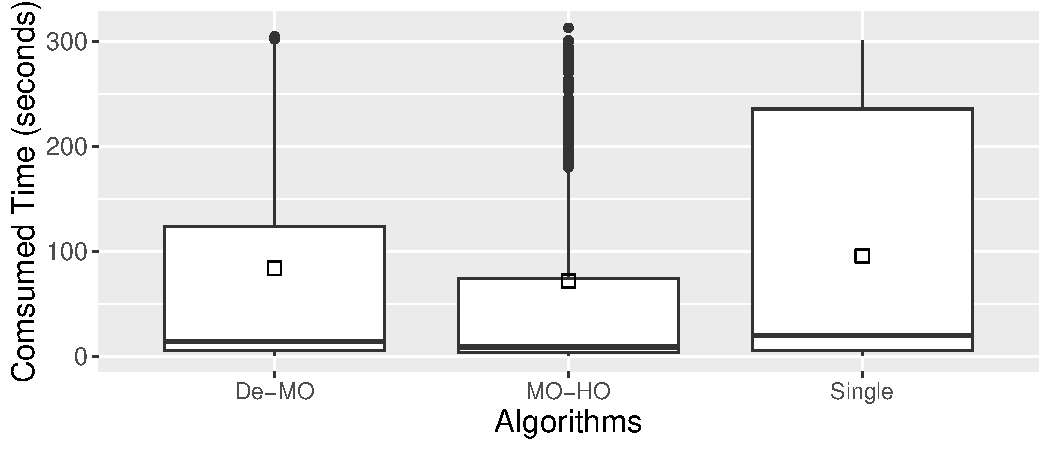
\includegraphics[width=\linewidth]{papers/moho/figures/time-overall.pdf}
    % \Description{A boxplot presenting the budget consumption in seconds fo De-MO, MO-HO, and Single.}
    \caption{Overall budget consumption in seconds (log. scale). ($\square$) denotes the arithmetic mean and (---) is the median.}
    \label{fig:eval:results-rq2-overall}
\end{figure}


Figure \ref{fig:eval:results-rq2-overall} shows the time (in seconds) needed by the \moho and the state-of-the-art algorithms to successfully reproduce the crashes in our benchmark.
On average, the fastest algorithm is \moho, with an average search time of 71 seconds per crash replication. The median of its running time is lower than 10 seconds. The second fastest algorithm is \decomposition that, on average, uses 84 seconds to reproduce the crashes. The slowest algorithm is \SGGA, which demands, on average, about 100 seconds. 

Moreover, the biggest improvements achieved by \moho in terms of efficiency are for \textit{XWIKI-14599}, in which \moho requires only 3\% of the time required by \SGGA to achieve crash reproduction, and \textit{MATH-3b}, in which \moho requires only 7\% of the time required by \decomposition to finish the crash reproduction task.
However, the biggest efficiency losses by \moho are in \textit{MATH-81b} with 45 seconds drop (15\% of time budget) and \textit{  XRENDERING-481} with 145 seconds drop (48\% of time budget) compared to \SGGA and \decomposition, respectively.

\begin{table}[t]
    \centering
    \caption{Pairwise comparison of the budget consumption with a small (S), medium (M), and large (L) effect size $\textit{\^{A}}_{12} < 0.5$ and a statistical significance $<0.05$.}
    \label{tab:efficiency}
    % \begin{smaller}
    \begin{tabular}{ l | c c c | c c c | c c c }
\hline 
\textbf{$\#(\textit{\^{A}}_{12} < 0.5)$}&\multicolumn{3}{c}{\textbf{Single}}&\multicolumn{3}{c}{\textbf{De-MO}}&\multicolumn{3}{c}{\textbf{MO-HO}}\\ 
 & L & M & S& L & M & S& L & M & S \\ 
\hline 
\textbf{Single}&-&-&-&7&-&4&1&-&2\\ 
\textbf{De-MO}&13&7&2&-&-&-&3&2&-\\ 
\textbf{MO-HO}&35&6&2&33&10&4&-&-&-\\ 
\hline
\end{tabular}
    % \end{smaller}
\end{table}

Table \ref{tab:efficiency} compares the budget consumption of the algorithms from a statistical point of view, \ie according to the effect sizes ($\textit{\^{A}}_{12} < 0.5$) and statistical significance ($\textit{p-value} < 0.5$). According to this table, \moho is the fastest algorithm: it significantly reproduced 43 (34.6\% of crashes) and 47 (37.9\% of crashes) crashes faster than \SGGA and \decomposition, respectively. Most of these significant improvements have large effect sizes (35 against \SGGA and 33 against \decomposition). In cases that \moho improves efficiency, on average, this algorithm decreases the time required for crash reproduction by 47\% and 58\% compared to \decomposition and \SGGA, respectively. 

Furthermore, Table \ref{tab:efficiency} shows a few cases, in which \moho increases the consumed time compared to the state-of-the-art: 3 against \SGGA and 5 against \decomposition. In most of these cases (7 out of 8), the crash reproduction process needs to reproduce a crash with only one frame. Even the exceptional case is a stack trace with three frames. In contrast, in cases that \moho wins, we have many crashes with more frames (six frames, for instance). Also, this table shows that \decomposition is significantly slower than \SGGA  in 11 crashes. Meanwhile, \moho is only slow in reproducing three crashes.
Hence, our proposed algorithm reduces the cases in which the multi-objectivization search process is slower than the single objective search by 73\%.

% Furthermore, Table \ref{tab:efficiency} shows that \decomposition significantly increases the speed of \SGGA in 7 crashes (6 with large effect size), while it is significantly slower than \SGGA in one crash.
% There is no statistically significant difference between these two algorithms in the remaining (large majority of) crashes.

\textbf{Summary (RQ$_3$). }
\textit{The fastest crash reproduction algorithm is \moho with an average improvement in running time in 34.6\% of the crashes compared to the state of the art.
%On average, it achieved the highest efficiency for crash reproduction. The highest improvement achieved by \moho in reproducing a crash is 97\% and 92\% against \SGGA and \decomposition, respectively. Also, it improved the crash reproduction speed in, at least, 34.6\% of the crashes. However, there are few crashes, in which \moho is slower than other algorithms. By analyzing these cases, we can see that in most of them (7 out of 8), the crash reproduction process needs to reproduce only one frame.
}


\subsection{Corner Cases Analysis}
\label{sec:results:corner}

Despite the notable improvements achieved by \moho, there are few specific cases, in which \SGGA or \decomposition outperform \moho. For instance, in Section \ref{sec:results:rq2}, \SGGA and \decomposition reproduce two crashes that are not reproduced by \moho. Also, we observed in Section \ref{sec:results:rq3} that the efficiency of these two algorithms is higher than \moho in 8 crashes.

To understand why \moho is counter-productive in a few cases, we performed a manual analysis to analyze the factors in \moho that negatively impact the crash reproduction process. Results of our analysis point to two adverse factors: \textbf{extra overhead in calculating the objectives (fitness evaluation)} and \textbf{helper-objectives misguidance}.



\begin{figure}[t]
    \begin{lstlisting}[numbers=left,
        firstnumber=0]
java.lang.ArrayIndexOutOfBoundsException: 2
    at org.apache.commons.math.linear.BigMatrixImpl.operate(BigMatrixImpl.java:997)
    \end{lstlisting}
    % \Description{The stack trace from the MATH-98b crash, composed of a thrown ArrayIndexOutOfBoundsException and the list of frames describing the active stack of method calls through which the exception propagated.}
    \caption{\texttt{MATH-98b} crash's stack trace \cite{just2014defects4j}.}
    \label{lst:factor1-stacktrace}
\end{figure}


\begin{figure}[t]
    \begin{lstlisting}[numbers=left,
        firstnumber=991,
        language=Java,
        basicstyle=\footnotesize]
public BigDecimal[] operate(BigDecimal[] v) {
    final int nRows = this.getRowDimension();
    final int nCols = this.getColumnDimension();
    final BigDecimal[] out = new BigDecimal[v.length];
    for (int row = 0; row < nRows; row++) {
        ...
        out[row] = sum; // <-- target line 
    }
    ...
}
    \end{lstlisting}
    % \Description{A code excerpt of the operate method mentioned in the MATH-98b crash.}
    \caption{Method \texttt{operate} appears in the first frame of the \texttt{MATH-98b} crash's stack trace \cite{just2014defects4j}.}
    \label{lst:factor1-code}
\end{figure}


\subsubsection{Extra calculation in fitness evaluation}
In some cases, crash reproduction is trivial, and the search process reproduces it in a few seconds. For instance, in \texttt{TIME-8b} \cite{just2014defects4j}, \SGGA and \decomposition reproduce the crash in about a second. The time required by \moho to reproduce this crash is three seconds (3 times more). This stems from the fact that fitness function evaluation in \moho is more time-consuming than the state-of-the-art: \SGGA and \decomposition need to calculate only the crash distance for each test case evaluation, while \moho needs to calculate the call diversity, as well. This extra calculation lengthens the search process by a couple of seconds. In these cases, the increased crash reproduction time is lower than 5 seconds, and it is negligible in practice.

\subsubsection{Helper-objectives misguidance}
In some other cases, the scenario, which leads to crash reproduction, needs a simple sequence of methods calls to the target class. Still, the complexity of this scenario stems from the input arguments used for the method calls. In these cases, since crash reproduction does not need the call diversity, \textit{method sequence diversity} objective misguides the search process. Alternatively, we need another objective for method input argument diversity (\ie improves the diversity of the input arguments for method calls). Adding new helper-objectives to consider other aspects of diversity is part of our future agenda. 

As an example, let us analyze \texttt{MATH-98b} (Figure \ref{lst:factor1-stacktrace}), in which MO-HO doubled the time consumed by the crash reproduction search process against state-of-the-art. This crash concerns an \texttt{ArrayIndexOutOfBounds\-Exception} .
Also, this crash has only one frame. For reproducing this crash, the generated test case needs to instantiate a class called \texttt{BigMatrixImpl} and call a method named \texttt{operate} (Figure \ref{lst:factor1-code}) with precise input values. Method \texttt{getColumnDimension} used in \texttt{operate} returns the number of rows in the data variable, which has been set in the constructor. To reproduce this crash, the generated test case should pass an array with a size smaller than the passed size to the constructor. In this case, method argument diversity could help the search process, and the method call diversity is not helpful.